% \begin{frame}[t]{Link Traversal-based Query Processing}
%     \begin{itemize}
%         \item Link Traversal iteratively dereferences data to query over
%         \item Continuously produces results
%         \item Can enforce fine-grained (document-level) access-control
%     \end{itemize}
% \end{frame}
% NOTES:
%   - Make the first seed document small so it stays same size throughout animation
%   - More justification on why link traversal for these environments

\begin{frame}{Link Traversal: Seed Document}
    \begin{columns}[T] % T aligns columns at the top
        % Left column: Image
        \begin{column}{0.6\textwidth} % Adjust width as needed
            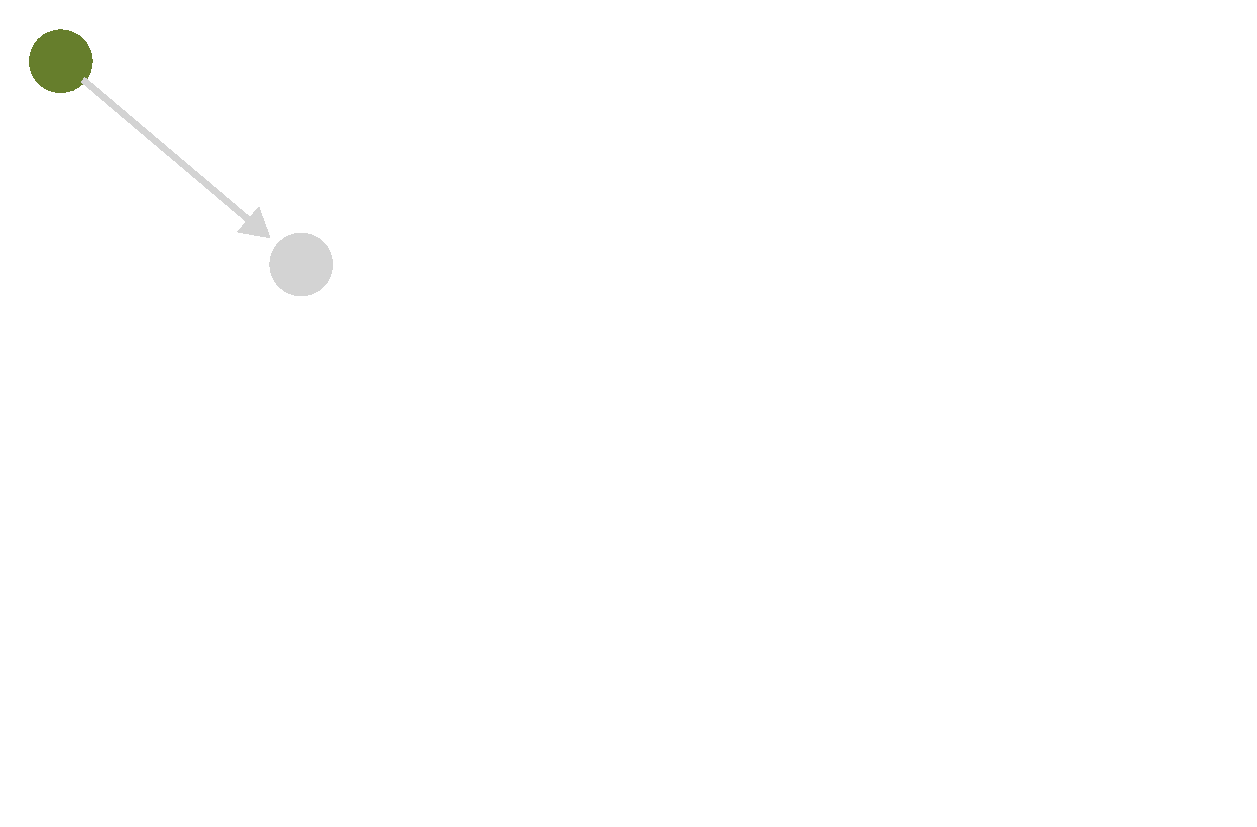
\includegraphics[width=\linewidth]{images/showing-link-traversal-step-0.pdf} % replace with your image file
        \end{column}

        % Right column: Text
        \begin{column}{0.4\textwidth} % Adjust width as needed
            \begin{itemize}
                \item Link Traversal starts from seed documents (URIs)
                \item These are provided by the user or in the query.
            \end{itemize}
        \end{column}
    \end{columns}
\end{frame}

\begin{frame}{Link Traversal: Traversal}
    \begin{columns}[T] % T aligns columns at the top
        % Left column: Image
        \begin{column}{0.6\textwidth} % Adjust width as needed
            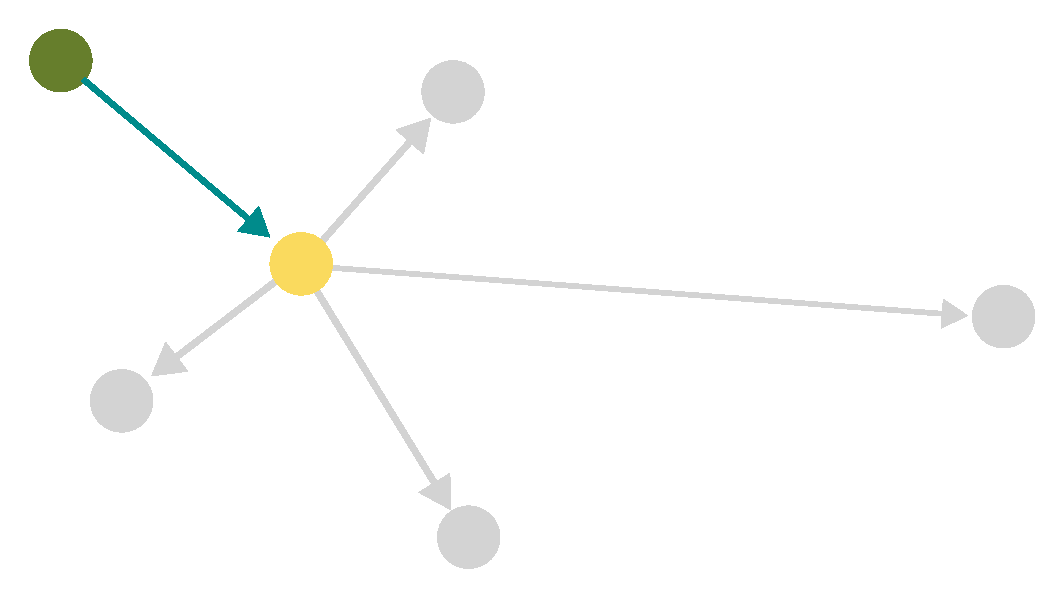
\includegraphics[width=\linewidth]{images/showing-link-traversal-step-1.pdf} % replace with your image file
        \end{column}

        % Right column: Text
        \begin{column}{0.4\textwidth} % Adjust width as needed
            \begin{itemize}
                \item New URIs are extracted from the seed document
                \item URIs are extracted in accordance with reachability criterions
            \end{itemize}
        \end{column}
    \end{columns}
\end{frame}


\begin{frame}{Link Traversal: Traversal}
    \begin{columns}[T] % T aligns columns at the top
        % Left column: Image
        \begin{column}{0.6\textwidth} % Adjust width as needed
            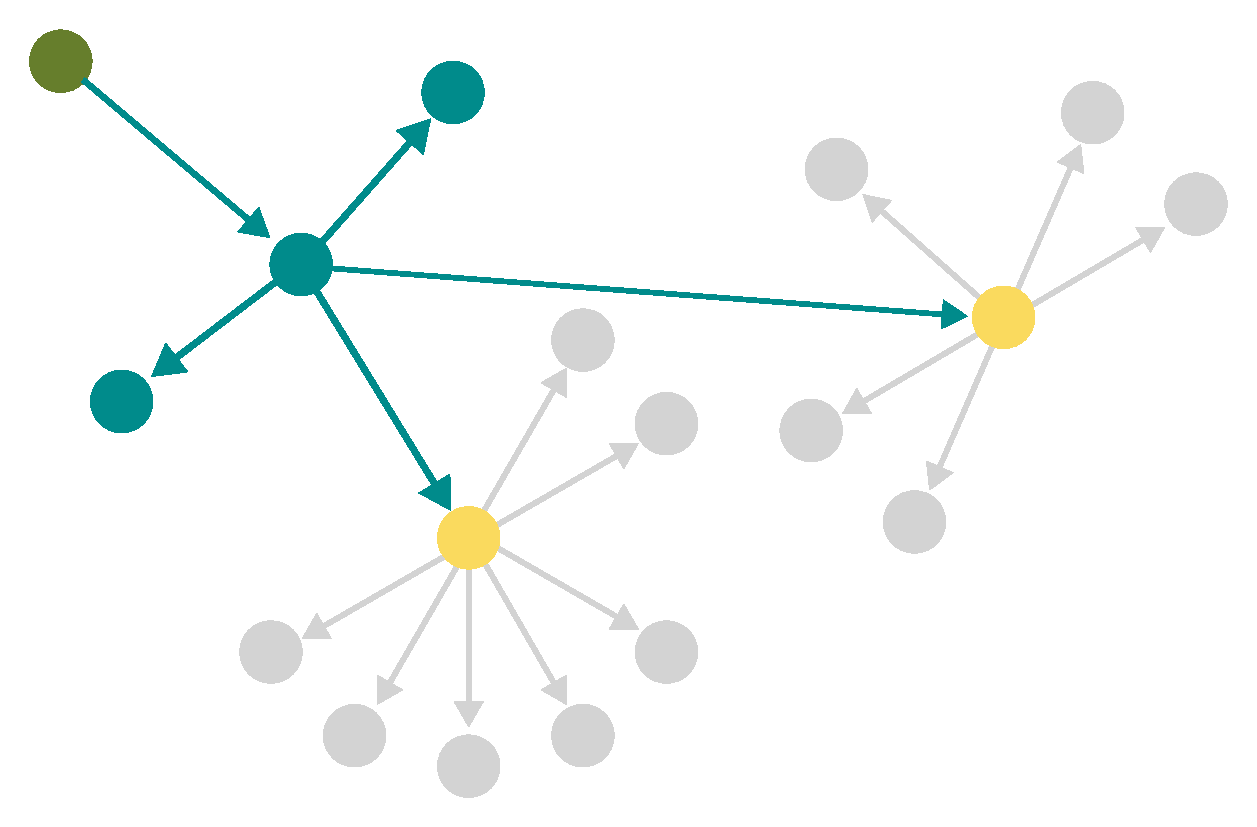
\includegraphics[width=\linewidth]{images/showing-link-traversal-step-2.pdf} % replace with your image file
        \end{column}

        % Right column: Text
        \begin{column}{0.4\textwidth} % Adjust width as needed
            \begin{itemize}
                \item New URIs are dereferenced and the process is repeated
            \end{itemize}
        \end{column}
    \end{columns}
\end{frame}



\begin{frame}{Link Traversal: Termination}
    \begin{columns}[T] % T aligns columns at the top
        % Left column: Image
        \begin{column}{0.6\textwidth} % Adjust width as needed
            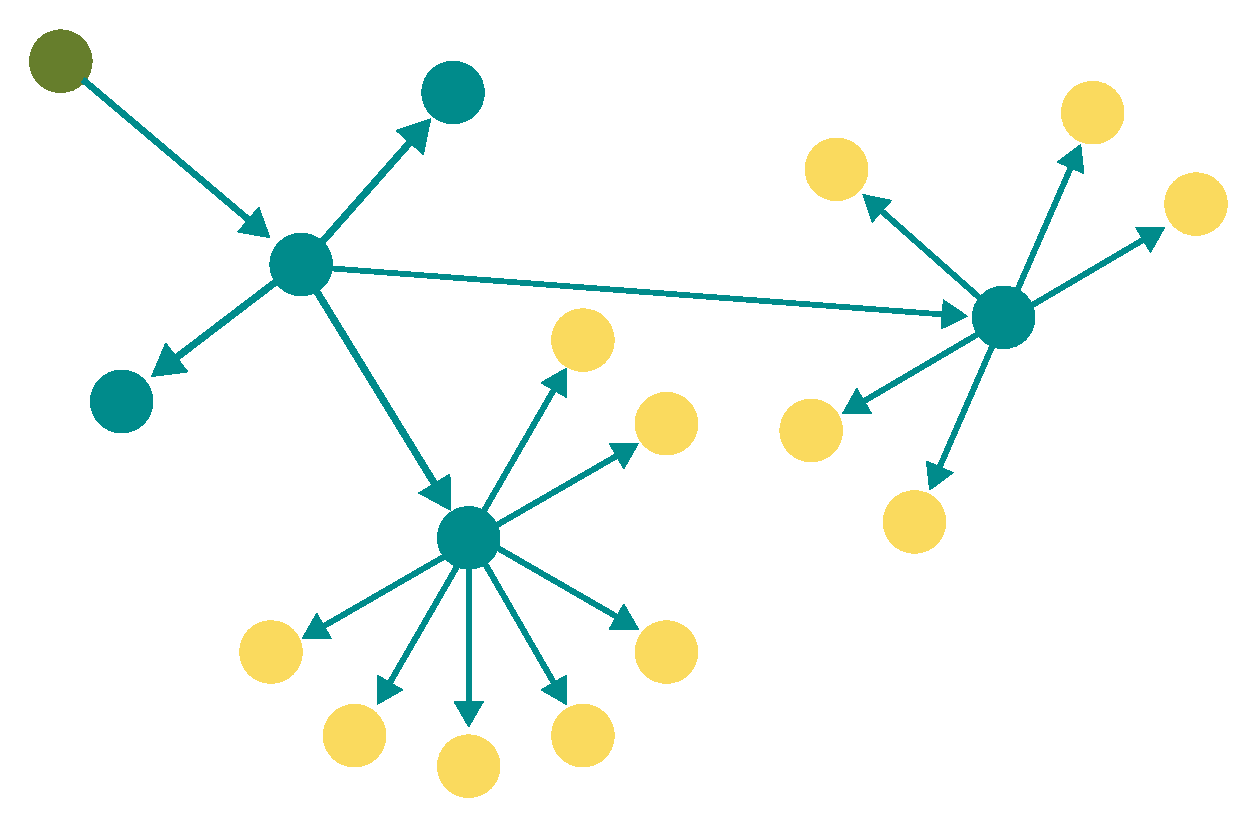
\includegraphics[width=\linewidth]{images/showing-link-traversal-step-3.pdf} % replace with your image file
        \end{column}

        % Right column: Text
        \begin{column}{0.4\textwidth} % Adjust width as needed
            \begin{itemize}
                \item This continues until all links are dereferenced
                \item Continuously produces results
                \item Can enforce fine-grained (document-level) access-control

            \end{itemize}
        \end{column}
    \end{columns}
\end{frame}